\documentclass[journal]{IEEEtran}

% Additional packages
\usepackage{graphicx}
\usepackage{amsmath}
\usepackage{lipsum}
\usepackage{hyperref} 
\usepackage{qrcode}
\usepackage{float}


\begin{document}

\title{Ohm’s Law and Thermistor Experiment}
\author{IBRAHIM H.I. ABUSHAWISH\\
ISTANBUL UNIVERSITY
FACULTY OF SCIENCE
DEPARTMENT OF PHYSICS \\
Instructor:  \\ % This can be updated easily
Experiment Date: 14.10.2024 , Report Submission Date: 21.10.2024 \\
Course \& Section Number: PHYS2305}

\maketitle

\maketitle

\begin{abstract}
This report presents an experimental investigation of Ohm's Law and the use of a thermistor for temperature measurement. Ohm's Law is applied to measure unknown resistances using a circuit consisting of known resistors, and equivalent resistances in series and parallel connections are explored. Additionally, the experiment demonstrates the relationship between temperature and resistance in a thermistor, a sensor used widely in temperature-sensitive applications. The objective is to verify the theoretical concepts of Ohm's Law and thermistor behavior under varying temperature conditions.
\end{abstract}

\section{Introduction}
The objective of this experiment is to study the relationship between current, voltage, and resistance as governed by Ohm’s Law, and to explore how resistance changes with temperature in a thermistor. Understanding these relationships is crucial for the design and analysis of electrical circuits and temperature sensing devices.

Ohm's Law defines the relationship between the voltage (V), current (I), and resistance (R) in an electrical circuit as:
\begin{equation}
    R = \frac{V}{I}
\end{equation}
This principle helps in determining unknown resistance values by measuring the current flowing through a circuit with a known voltage.

Thermistors, which are temperature-sensitive resistors, exhibit a change in resistance with temperature. Depending on the type of thermistor, the relationship between resistance and temperature can either be direct or inverse. In this experiment, we will use a Negative Temperature Coefficient (NTC) thermistor, where resistance decreases as temperature increases.

\section{Theory}
\subsection{Ohm's Law}
Ohm’s Law states that the current passing through a conductor between two points is directly proportional to the voltage across the two points. The resistance is the constant of proportionality in this relationship. Mathematically, this can be expressed as:
\begin{equation}
    V = IR
\end{equation}
where \( V \) is the voltage (in volts), \( I \) is the current (in amperes), and \( R \) is the resistance (in ohms).

For circuits with resistors in series, the equivalent resistance is the sum of all resistances:
\begin{equation}
    R_{\text{eq}} = R_1 + R_2 + \dots + R_n
\end{equation}

For resistors in parallel, the equivalent resistance is given by:
\begin{equation}
    \frac{1}{R_{\text{eq}}} = \frac{1}{R_1} + \frac{1}{R_2} + \dots + \frac{1}{R_n}
\end{equation}

\subsection{Thermistors}
A thermistor is a type of resistor whose resistance changes significantly with temperature. The relationship between temperature and resistance in a thermistor can be expressed by the following equation:
\begin{equation}
    R = R_0 (1 + \alpha \Delta T)
\end{equation}
where \( R_0 \) is the initial resistance, \( \alpha \) is the temperature coefficient of resistance, and \( \Delta T \) is the change in temperature.

Thermistors are classified into two types:
\begin{itemize}
    \item Negative Temperature Coefficient (NTC): Resistance decreases as temperature increases.
    \item Positive Temperature Coefficient (PTC): Resistance increases as temperature increases.
\end{itemize}

In this experiment, an NTC thermistor is used to measure the temperature by observing the change in resistance as the water temperature rises.

\section{Experimental Setup}
\subsection{Ohm's Law Experiment}
In this experiment, we investigate the validity of Ohm’s Law by measuring the current through different resistors at a constant voltage. The experimental setup includes a voltage source, an ammeter to measure the current, and resistors connected in series and parallel.

The circuit diagram used in the experiment is shown in Figure~\ref{fig:ohmslaw}.

\begin{figure}[H]
    \centering
    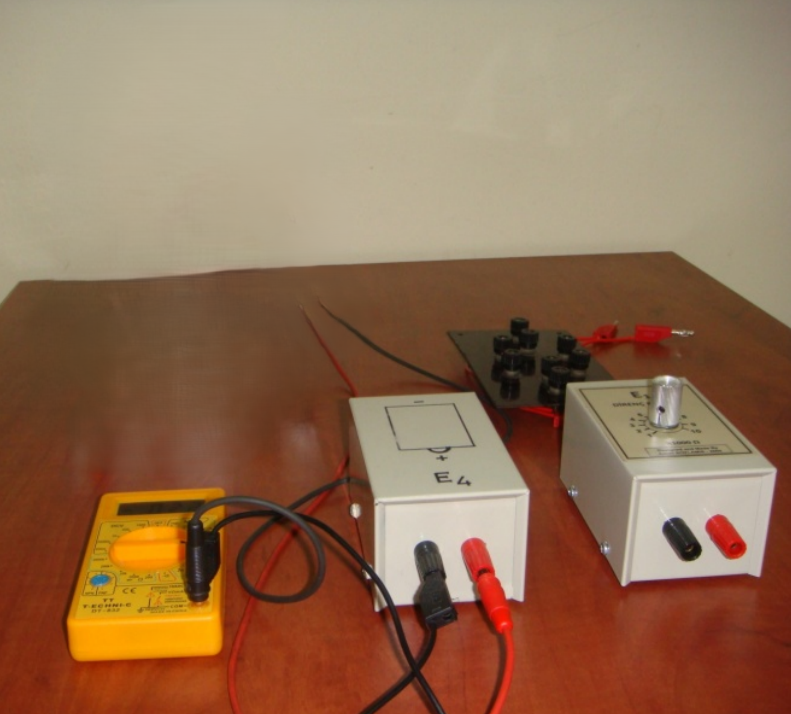
\includegraphics[width=0.45\textwidth]{IMAGES/Ohms_Law_Setup_only.png} % Placeholder, replace with actual image
    \caption{Ohm's Law Experimental Setup}
    \label{fig:ohmslaw}
\end{figure}

A known voltage is applied across a resistor, and the current passing through the circuit is measured using an ammeter. By plotting a graph of current versus resistance, we verify Ohm’s Law and calculate the equivalent resistances for both series and parallel connections.

\subsection{Thermistor Experiment}
The thermistor experiment involves measuring the resistance of a thermistor as the temperature of the surrounding water is increased. A power supply is used to maintain a constant voltage across the thermistor. The resistance is calculated using the current measured by a milliammeter. 

The experimental setup for the thermistor experiment is shown in Figure~\ref{fig:thermistor}.

\begin{figure}[H]
    \centering
    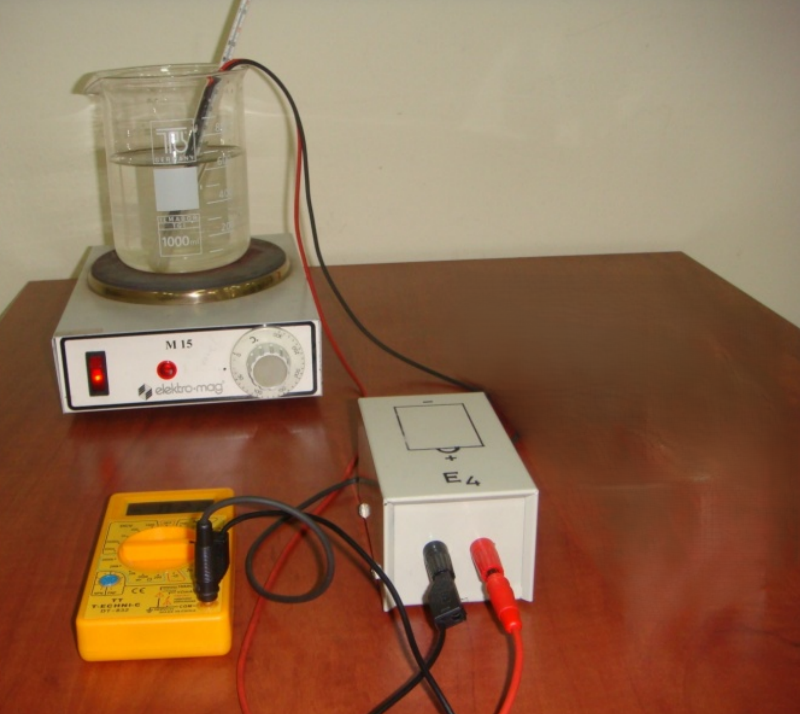
\includegraphics[width=0.45\textwidth]{IMAGES/Thermistor_Setup.png} % Placeholder, replace with actual image
    \caption{Thermistor Experimental Setup}
    \label{fig:thermistor}
\end{figure}

As the water is heated in steps of 5°C, the current is recorded and the resistance is calculated using Ohm’s Law. A graph of resistance versus temperature is plotted to analyze the behavior of the thermistor.

\section{Procedure}
\subsection{Ohm’s Law Experiment Procedure}
\begin{enumerate}
    \item Construct the circuit as shown in Figure~\ref{fig:ohmslaw}, with a known resistor connected in series with the voltage source and ammeter.
    \item Measure the current for each resistor value and record the data.
    \item Repeat the measurements for resistors connected in parallel.
    \item Plot the graph of current versus resistance and use the data to calculate the unknown resistances.
\end{enumerate}

\subsection{Thermistor Experiment Procedure}
\begin{enumerate}
    \item Connect the thermistor in the circuit as shown in Figure~\ref{fig:thermistor}.
    \item Measure the initial temperature of the water and the corresponding current through the thermistor.
    \item Gradually heat the water in 5°C increments, measuring the current at each step.
    \item Calculate the resistance at each temperature using Ohm’s Law.
    \item Plot the graph of resistance versus temperature and analyze the behavior of the thermistor.
\end{enumerate}

\section{Results and Analysis}
\textit{[This section will include the data tables and graphs from the calculations and measurements once they are available.]}

\section{Discussion}
\textit{[This section will discuss the results, including any deviations from theoretical expectations, possible sources of error, and interpretations based on the graphs and tables generated from the data. Calculations for series and parallel circuits, as well as the thermistor behavior, will be examined.]}

\section{Conclusion}
This experiment successfully demonstrated Ohm’s Law by measuring the relationship between current, voltage, and resistance. The equivalent resistances for series and parallel connections were calculated and verified through measurement. Furthermore, the thermistor experiment showed how resistance decreases as temperature increases in an NTC thermistor. This behavior aligns with theoretical predictions, highlighting the effectiveness of thermistors in temperature measurement applications.

\section{Additional Resources}
For detailed information, including the Lab Manual, source code, and related experiments, visit the GitHub repository provided below or scan the QR code in Fig.~\ref{fig:qr}.

\begin{thebibliography}{9}

\bibitem{lab_manual}
    ISTANBUL UNIVERSITY, 
    \textit{Physics Laboratory II Experiment Book: Electricity and Magnetism}, 
    Department of Physics, 2024.

\bibitem{github}
    \textit{Source code and additional experiments are available in the GitHub repository.} \\ 
    Access it at: \url{https://github.com/ibeuler/LAB-Reports}

\end{thebibliography}

\begin{figure}[H]
    
    \centering
    \begin{minipage}{0.15\textwidth}
        \centering
        \qrcode[height=2cm]{https://github.com/ibeuler/LAB-Reports}
    \end{minipage}%
    \begin{minipage}{0.2\textwidth}
        \raggedright
        \caption{Access the GitHub repository for the lab manual, source code, and related experiments: \href{https://github.com/ibeuler/LAB-Reports}{\url{https://github.com/ibeuler/LAB-Reports}}.}
    \end{minipage}
    \label{fig:qr}
\end{figure}


\end{document}
